% CVPR 2022 Paper Template
% based on the CVPR template provided by Ming-Ming Cheng (https://github.com/MCG-NKU/CVPR_Template)
% modified and extended by Stefan Roth (stefan.roth@NOSPAMtu-darmstadt.de)

\documentclass[11pt,twocolumn,letterpaper]{article}
% \documentclass[11pt,twocolumn,a4paper]{article}

%%%%%%%%% PAPER TYPE  - PLEASE UPDATE FOR FINAL VERSION
\usepackage[pagenumbers]{cvpr}      % To produce the REVIEW version
%\usepackage{cvpr}              % To produce the CAMERA-READY version
%\usepackage[pagenumbers]{cvpr} % To force page numbers, e.g. for an arXiv version

% Include other packages here, before hyperref.
\usepackage{graphicx}
\usepackage{amsmath}
\usepackage{amssymb}
\usepackage{booktabs}
\usepackage{multirow}
\usepackage{hyperref}

% \usepackage{authblk}

% It is strongly recommended to use hyperref, especially for the review version.
% hyperref with option pagebackref eases the reviewers' job.
% Please disable hyperref *only* if you encounter grave issues, e.g. with the
% file validation for the camera-ready version.
%
% If you comment hyperref and then uncomment it, you should delete
% ReviewTempalte.aux before re-running LaTeX.
% (Or just hit 'q' on the first LaTeX run, let it finish, and you
%  should be clear).
\usepackage[pagebackref,breaklinks,colorlinks]{hyperref}


% Support for easy cross-referencing
\usepackage[capitalize]{cleveref}
\crefname{section}{Sec.}{Secs.}
\Crefname{section}{Section}{Sections}
\Crefname{table}{Table}{Tables}
\crefname{table}{Tab.}{Tabs.}


%%%%%%%%% PAPER ID  - PLEASE UPDATE
\def\cvprPaperID{616} % *** Enter the CVPR Paper ID here
\def\confName{CVPR}
\def\confYear{2022}

\begin{document}

%%%%%%%%% TITLE - PLEASE UPDATE
\title{COMP3425 Assignment 2}

\author{
    Zhiyuan Chen\\
    Microsoft Research\\  % \quad The Australian National University\\
    {\tt\small zyc.ai}
%  \and
%    Nuonuo F.C. Yang\\
%    Shanghai Artificial Intelligence Laboratory\\
%  \and
%    GPT-3\\
%    OpenAI\\
%    {\tt\small openai.com}
}

% \author[1]{Alice Smith}
% \author[2]{Bob Jones}
% \affil[1]{Department of Mathematics, University X}
% \affil[2]{Department of Biology, University Y}

% For a paper whose authors are all at the same institution,
% omit the following lines up until the closing ``}''.
% Additional authors and addresses can be added with ``\and'',
% just like the second author.
% To save space, use either the email address or home page, not both
\maketitle

%%%%%%%%% ABSTRACT
\begin{abstract}
In this work, we study the COVID-19 attitudes and behaviours in Australia~\cite{data}.
Part of codes of this work is available at: \url{http://github.com/ZhiyuanChen/COMP3425-ass2}.
\end{abstract}

%%%%%%%%% BODY TEXT
\section{Platform}

For this work, we used three different machines: a development node~\ref{node:dev}, a computation node~\ref{node:comp}, and a multi-functional node~\ref{node:multi}.
All of them are running Ubuntu 20.04 LTS.
We use Python in this work.
For better reproducibility, all random seeds are fixed to 1031.

\subsection{Development Node}\label{node:dev}

The development node is a Standard\_NC24ads\_A100\_v4 virtual machine on Azure.
It has 24 vCPU cores of a AMD EPYC 7V13 CPU, 220 GiB memory, and a NVIDIA Tesla A100 GPU with 80 GiB GPU memory.

\subsection{Computation Node}\label{node:comp}

The computation node is a NVIDIA DGX Station.
It has one Intel Xeon E5-2698v4 CPU with 20 cores, 256 GiB memory, and 4 NVIDIA Tesla V100 GPU with 32 GiB GPU memory each.

\subsection{Multi-functional Node}\label{node:multi}

The multi-functional node is a Standard\_NC24rs\_v3 virtual machine on Azure.
It has 24 vCPU cores of a Intel Xeon CPU E5-2690v4 CPU, 448 GiB memory, and 4 NVIDIA Tesla V100 GPU with 16 GiB GPU memory each.

\section{Data}

\subsection{Collection}\label{collection}

In this work, we study a poll dataset of COVID-19 attitudes and behaviours in Australia~\cite{data}.
It is the 35\textsuperscript{th} of a series of polls organised by the Social Research Center for the ANU.
This dataset is collected in August 2020, building upon the previous data collected in January, April, and May.
The dataset composes political opinions, experience with COVID-19, opinions and behavioral responses to COVID-19 vaccines, mental health status, activities and employments, opinions and behavioral responses to bushfire, etc.

In this work, we focus on a selected subset of the original data.
We mainly work on the opinion of the responses, while all detailed information, for example, the occupation are ignored.

\subsection{Correlation}\label{correlation}

\begin{figure}[htb]
    \centering
    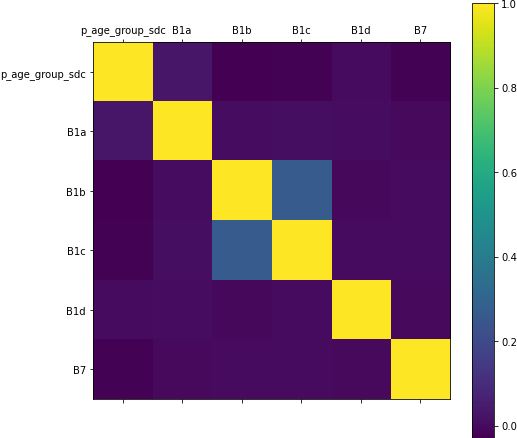
\includegraphics[width=1\linewidth]{assests/data.png}
    \caption{The Pearson product-moment correlation amongst $p\_age\_group\_sdc$, $B1_a$, $B1_b$, $B1_c$, $B1_d$, and $B7$.}
    \label{fig:data}\vspace{-2.5mm}
\end{figure}

In this section we studies the pairwise correlation amongst of the dataset.
Figure~\ref{fig:data} illustrated the Pearson correlation amongst $p\_age\_group\_sdc$, $B1_a$, $B1_b$, $B1_c$, $B1_d$, and $B7$.

The meaning of each feature is listed as follows:

\begin{itemize}
  \vspace{-2.5mm}\item[$B1_a$] If has been tested for COVID-19
  \vspace{-2.5mm}\item[$B1_b$] If has had close contact with confirmed infection of COVID-19
  \vspace{-2.5mm}\item[$p\_age\_group\_sdc$] Age group as of April 2020
  \vspace{-2.5mm}\item[$B1_c$] If has had close contact with possible infection of COVID-19
  \vspace{-2.5mm}\item[$B1_d$] If feels worried for the safety
  \vspace{-2.5mm}\item[$B7$] Opinions on PPE~\footnote{Personal Protective Equipment} in public space
\end{itemize}

We can observe that $B1_b$ and $B1_c$ are weakly correlated, with a Pearson correlation of 0.26.
All other variables are independent of each other.

The correlation between $B1_b$ and $B1_c$ is anticipated as they both indicates the contacts of COVID-19 infections.

We also expected the correlation between $B1_a$, $B7$ and $p\_age\_group\_sdc$, as we thought the opinions on testing and PPE is related to age group.
However. it is not presented.

When we take a broader look of the dataset, as shown in figure~\ref{fig:all}, there are much more correlations.
$A4_a$ to $A4_f$ are weakly correlated with an average Pearson of 0.35.
$D1_a$ to $D1_f$ are also weakly correlated with an average Pearson of 0.47, while correlation between $D1_a, D1_b$, and $D1_c, D1_d$ exceeds 0.6.
$E1_a$ to $E1_f$, $F1$s, and $F2$s are correlated with an average Pearson of around
0.6.

\begin{figure}[htb]
    \centering
    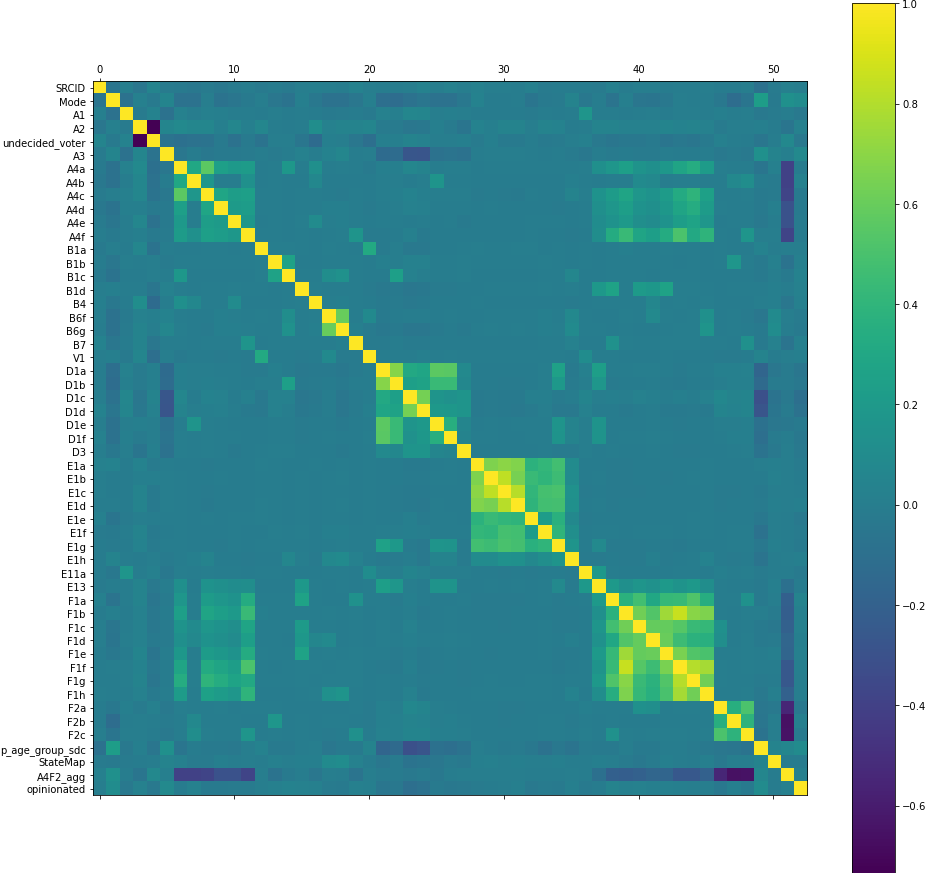
\includegraphics[width=1\linewidth]{assests/all.png}
    \caption{The Pearson product-moment correlation amongst all cols in 3425\_data.csv.}
    \label{fig:all}\vspace{-2.5mm}
\end{figure}

\section{Direction of Austlia}\label{direction}

We studies the association between other responses and the feeling of the direction of Australia in this section.

For the $55$ features, we construct a total of $303$ one-hot encoding and perform association mining.

We use FP-growth algorithm~\cite{fpgrowth} to search for association rules.
Although FP-growth generally costs more memory than conventional algorithms such as Apriori~\cite{apriori} because it takes memory to construct FP Trees.
However, in our experiment, since there are many features, Apriori algorithm~\cite{apriori} starts to run into Out Of Memory issues when $min\_support$ is set to $0.2$.

\begin{table*}[htb!]
\resizebox{2.1\columnwidth}{!}{
\begin{tabular}{lllllllll}
\toprule
antecedents               & consequents & a support & c support & support  & confidence & lift     & leverage & conviction \\
\midrule
(B1b\_2)                  & (A1\_2)     & 0.9856           & 0.6161           & 0.6080 & 0.6168   & 1.0011 & 0.0007 & 1.0018   \\
(E1d\_2)                  & (A1\_2)     & 0.9500           & 0.6161           & 0.5900 & 0.6210   & 1.0080 & 0.005 & 1.0129   \\
(ud\_voter\_F) & (A1\_2)     & 0.9474           & 0.6161           & 0.5897 & 0.6224   & 1.0102 & 0.0059 & 1.0166   \\
(E1c\_2)                  & (A1\_2)     & 0.9484           & 0.6161           & 0.5880 & 0.6200   & 1.0063 & 0.0037 & 1.0103    \\
(B1c\_2)                  & (A1\_2)     & 0.9428           & 0.6161           & 0.5831 & 0.6185   & 1.0038 & 0.0022 & 1.0062   \\
(E1e\_2)                  & (A1\_2)     & 0.9278           & 0.6161           & 0.5815 & 0.6268   & 1.0172  & 0.0099 & 1.0285   \\
(E1b\_2)                  & (A1\_2)     & 0.9069           & 0.6161           & 0.5609 & 0.6185   & 1.0039 & 0.0022 & 1.0062   \\
(Mode\_1)                 & (A1\_2)     & 0.9409           & 0.6161           & 0.5835 & 0.6201   & 1.0065 & 0.0038 & 1.0105  
\bottomrule
\end{tabular}}
\vspace{-1mm}
    \caption{Antecedents of consequents $A2$, with a $min\_support$ of 0.55 and a $min\_confidence$ of 0.61. $a support$ refers to support of antecedents, $c support$ refers to support of consequents, and $ud\_voter\_F$ refers to $undecided\_voter=False$.}
\label{tab:direction}\vspace{-3mm}
\end{table*}

We start with a standard value, $0.5$ for both min\_support and min\_confidence. However, out of the $1051859$ association rules, there were only consequents for satisfactory ($A1=2$).
We further tuned $min\_support$ to $0.2$, generated $1627406$ frequent item set and over $200000000$ association rules, however, there it still no consequents for very satisfactory ($A1=1$).
The program crashed before we have the chance to explore other consequents.
We did not continue to try to find the association of other satisfactory status and focus on satirfactory ($A1=2$).

After tuning, we adopt a $min\_support=0.55$ and $min\_confidence=0.61$, there were a total of 51 association rules, a selected portion of the important antecedents are listed in table~\ref{tab:direction}.

We believe the association mining could be a useful technique on thin data.
Most of the data are categorical variables and can be easily transformed to binaries data with one-hot encoding.
In addition, the data is from a survey, association minting could help us understand the inner connections of the answers of each question.
We argue that the unideal results could be improved with proper data processing, e.g. aggregate values.

\section{Opinionated}\label{opinionated}

\begin{table*}[htb!]
% Please add the following required packages to your document preamble:
% \usepackage{multirow}
\resizebox{2.1\columnwidth}{!}{
\begin{tabular}{@{}llllllllll@{}}
\toprule
&       & \multicolumn{2}{c}{Logistic Regression} & \multicolumn{2}{c}{SVM} & \multicolumn{2}{c}{Decision Tree} & \multicolumn{2}{c}{MLP} \\
&       & False               & True              & False       & True      & False            & True           & False       & True      \\
\midrule
\multirow{2}{*}{Groundtruth} & False  & 1730                & 168               & 1885      & 13        & 1898           & 0               & 1804      & 94        \\
& True & 940                 & 223               & 650         & 513       & 0               & 1163           & 117       & 1046     
\bottomrule
\end{tabular}}
\vspace{-1mm}
    \caption{Confusion Matrix of different models in classifying $Opinionated$. Values are sum over $10$-fold evaluations.}
\label{tab:opinionated:confusion}\vspace{-3mm}
\end{table*}

\begin{table}[htb]
\resizebox{\columnwidth}{!}{
\begin{tabular}{@{}lcccc@{}}
\toprule
      & LR      & SVM    & DTree & MLP    \\
\midrule
AUROC & 0.5539  & 0.7168 & 1     & 0.9252 \\
F1    & 0.2874  & 0.6055 & 1     & 0.9079
\bottomrule
\end{tabular}}
\vspace{-1mm}
    \caption{Performance of different models in classifying $Opinionated$. Values are averaged over $10$-fold evaluations.}
\label{tab:opinionated:score}\vspace{-3mm}
\end{table}

In this section, we studies the performance amongst different machine learning algorithms on classifying the $Opinionated$.

The target, $Opinionated$ is a Boolean variable that aggregates $A4$s and $F2$s, indicating whether a subject is opinionated.

\begin{table*}[htb!]
% Please add the following required packages to your document preamble:
% \usepackage{multirow}
\resizebox{2.1\columnwidth}{!}{
\begin{tabular}{@{}llllllllll@{}}
\toprule
&       & \multicolumn{2}{c}{Logistic Regression} & \multicolumn{2}{c}{SVM} & \multicolumn{2}{c}{Decision Tree} & \multicolumn{2}{c}{MLP} \\
&       & False               & True              & False       & True      & False            & True           & False       & True      \\
\midrule
\multirow{2}{*}{Groundtruth} & False  & 1699                & 199               & 1820      & 78        & 1898           & 0               & 1804      & 94        \\
& True & 344                 & 819               & 378         & 785       & 0               & 1163           & 164       & 999     
\bottomrule
\end{tabular}}
\vspace{-1mm}
    \caption{Confusion Matrix of different models in classifying $Opinionated$, after data processing. Values are sum over $10$-fold evaluations.}
\label{tab:opinionated:confusion2}\vspace{-3mm}
\end{table*}

\begin{table}[htb]
\resizebox{\columnwidth}{!}{
\begin{tabular}{@{}lcccc@{}}
\toprule
      & LR      & SVM    & DTree & MLP    \\
\midrule
AUROC & 0.7986  & 0.8154 & 1     & 0.9042 \\
F1    & 0.7473  & 0.7716 & 1     & 0.8848
\bottomrule
\end{tabular}}
\vspace{-1mm}
    \caption{Performance of different models in classifying $Opinionated$, after data processing. Values are averaged over $10$-fold evaluations.}
\label{tab:opinionated:score2}\vspace{-3mm}
\end{table}

We compare the performance of Logistic Regression, SVM, Decision Tree, and MLP, the confusion matrix is demonstrated in table~\ref{tab:opinionated:confusion}.
All algorithms are using the default settings in sci-kit-learn, except $max\_iter$ are set to $100000$ to allow each classifier has enough training to converge.
We perform a $10$-fold evaluation for the robustness of thef result.
We use AUROC (area under receiver operating characteristic) and F1 to evaluate the performance, table~\ref{tab:opinionated:score} illustrated the results.

We further processed the original data, making class label organized in continuous integer, i.e. converted classes labeled as $(-99, -98, 1, 2, 3)$ to $(0, 1, 2, 3, 4)$.
We have gained a significant performance improvement, as shown in table~\ref{tab:opinionated:confusion2} and table~\ref{tab:opinionated:score2}.

Decision Tree achieved best result with no prediction error.
MLP outperform SVM and logistic regression by a large margin.
Although SVM shows promising results in terms of AUROC, it's F1 score in the original form is rather unsatisfactory, indicating issues in precision/recall.
Logistic Regression should have achieved a better result as our data is linearly separable, however, it's basically producing Brownian outputs in the original form.
Proper data processing is crucial to Logistic Regression and SVM.
Both Logistic Regression and SVM achieved an AUROC score of around $0.8$ in the processed form, with $44.18\%$ and $13.76\%$ improvement respectively.

\section{Satisfaction}\label{satisfaction}

In this section, we used a Transformer~\cite{transformer} to predict the satisfaction on feeling about life in general.

We formulate the task as a multi-class classification problem and use CrossEntropy to calculate loss.

Each input feature is considered as a word, except for $A1$, $A4F2\_agg$, and the targets $A3$.
We construct a sentences with a fixed length of $52$ words.
No internal normalization is performed on the word embedding.

We customised a BERT~\cite{bert} model for the prediction.
It consists $16$ layers of transformer encoder with $16$ heads, $1024$ embedding dim, and $4096$ feedforward dim.
We used position embedding described in TUPE~\cite{tupe}.
There is no complex neck design, we only have one fully-connected layer as prediction head.

We train the model for $100$ epochs using an AdamW optimizer with initial learning rate of $3\mathrm{e}{-4}$, cosine decay to $1\mathrm{e}{-8}$.
The weight decay is set to $0.01$, and we clip gradients over $1.0$.

As before, we perform a $10$-fold cross validation to evaluate our model, the average top-1 accuracy is $35.90\%$.

We argue that the low performance of the transformer is resulted by lack of pre-training.
And a simple pre-training of the network in a MLM (masked-language model) manner could have significant impact.
Besides, the training dataset is too small.
Although there was no sign of over-fitting, the model it self contains $220$ million trainable parameters, the dataset is just too small.

\section{Vote}\label{vote}

In this section, we studies if it is possible to predict whether a person is an $undecided\_voter$ or not.
Similar to $opinionated$, we use a $10$-fold validation to evaluate our model.
This time, we focus only on the non-linear algorithms (SVM, Decision Tree, and MLP).
To speed up searching, we use nni to perform grid search on the parameters.
$undecided\_voter$ is a highly imbalanced data.
Out of $3061$ population, only $161$ subjects is False.
We anticipate model will tends to predict False no matter the input without proper scaling.

We have tried both the original data and the processed data described in section~\ref{opinionated}, there it no significant performance gap.

\subsection{SVM}

The baseline performance of SVM is as expected, predict most values to be False.
The true positive is $0$, while false negative is $161$, AUROC is $0.4997$.

We tested different class weights to address the label imbalance issues, and found although set 'balanced' to class weights could alleviate the issues to some extent, manually setting positive weights to $20$ yields the best performance of SVM, with an AUROC of $0.5925$.

We also test different kernel functions, including poly and sigmoid.
Although poly works slightly better on default settings, it was outperformed by default rbf functions in balanced settings.
Further tunning on coef0 and degree does not contribute much.
The best poly function SVM achieves $0.5774$ when class weights is $3061/161$, coef0 is $1$ and degree is $6$.

Adjusting gamma and probability does not help.

\subsection{Decision Tree}

The baseline performance of Decision Tree is slightly better than SVM, with an AUROC of $0.5001$.

Setting class weights to $3061/161$ increases AUROC to $0.5177$, using random splitter further improves to $0.5291$, however, they still have no difference comparing to a random classifier.

We believe it could be a result of over-fitting, and set ccp\_alpha to $0.01$.
The result is $0.6172$, significantly better than previous attempts.

All other parameter do not contribute.

\subsection{MLP}

The baseline performance of MLP is $0.5134$.

By using Adam optimizer, setting stronger regularization (alpha=$0.001$), and use a smaller network with $20$ hidden\_layer\_size.

The influence of other parameters is not significant.

We argue that with a better neural network architecture, for example, as described in section~\ref{satisfaction}, we could achieve a better performance.
However, the time frame of this assignment prevents us for conducting more extensive experiments.

\section{Clustering}

In this selection, we use K-means algorithm to find if it is possible to cluster subjects into sub-groups, figure~\ref{fig:cluster} visualises the clustering results.

\begin{figure*}
     \centering
     \begin{subfigure}[b]{0.23\textwidth}
         \centering
         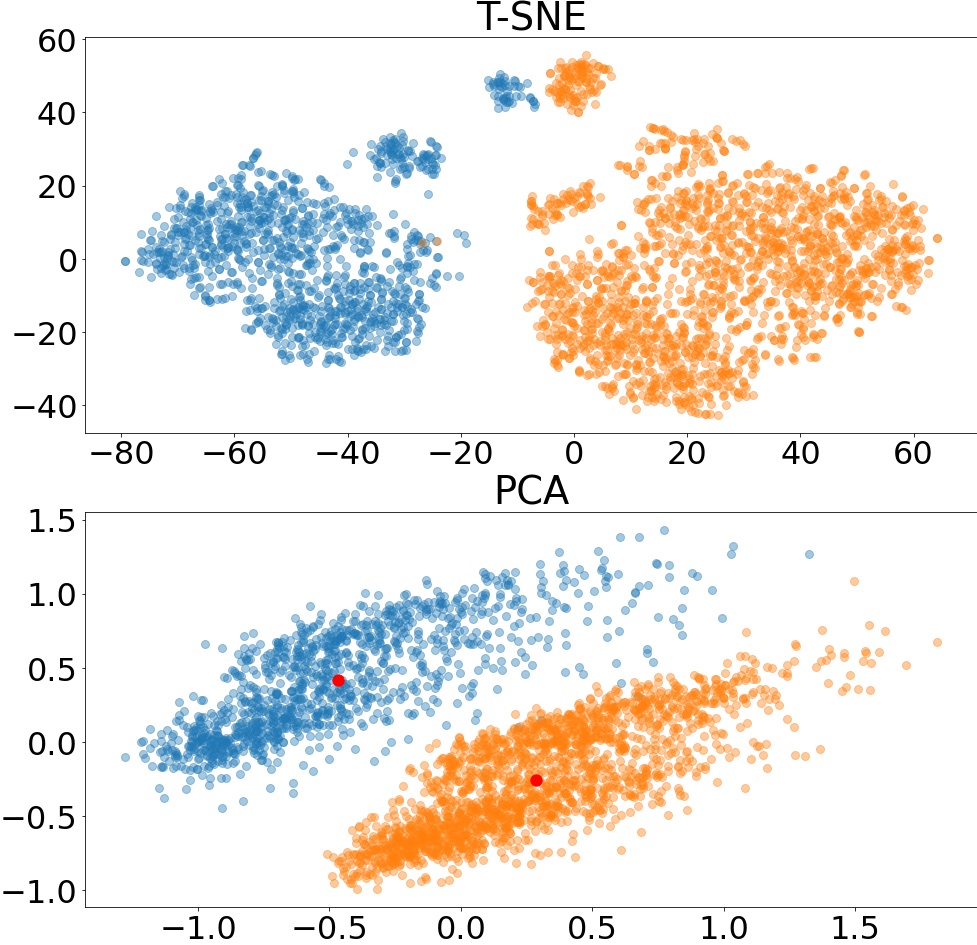
\includegraphics[width=\textwidth]{assests/2-means.png}
         \caption{2-Means}
         \label{fig:cluster:2means}
     \end{subfigure}
     \hfill
     \begin{subfigure}[b]{0.23\textwidth}
         \centering
         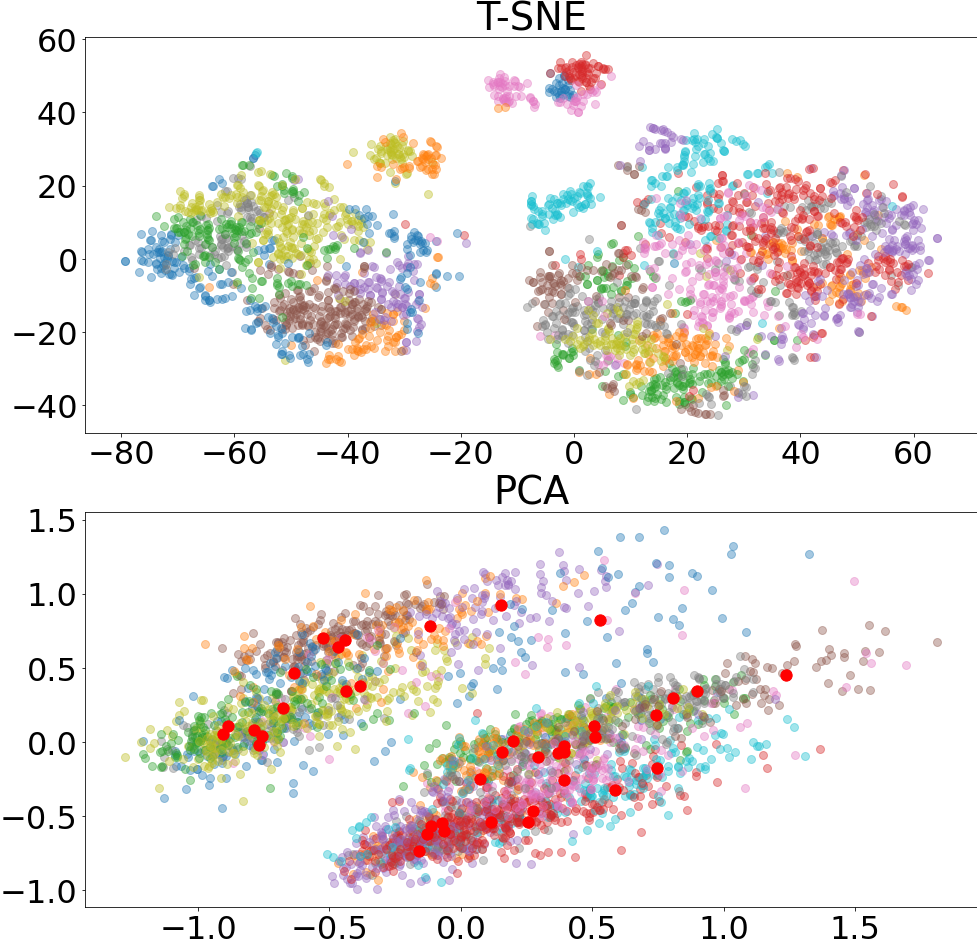
\includegraphics[width=\textwidth]{assests/39-means.png}
         \caption{39-Means}
         \label{fig:cluster:39means}
     \end{subfigure}
     \hfill
     \begin{subfigure}[b]{0.23\textwidth}
         \centering
         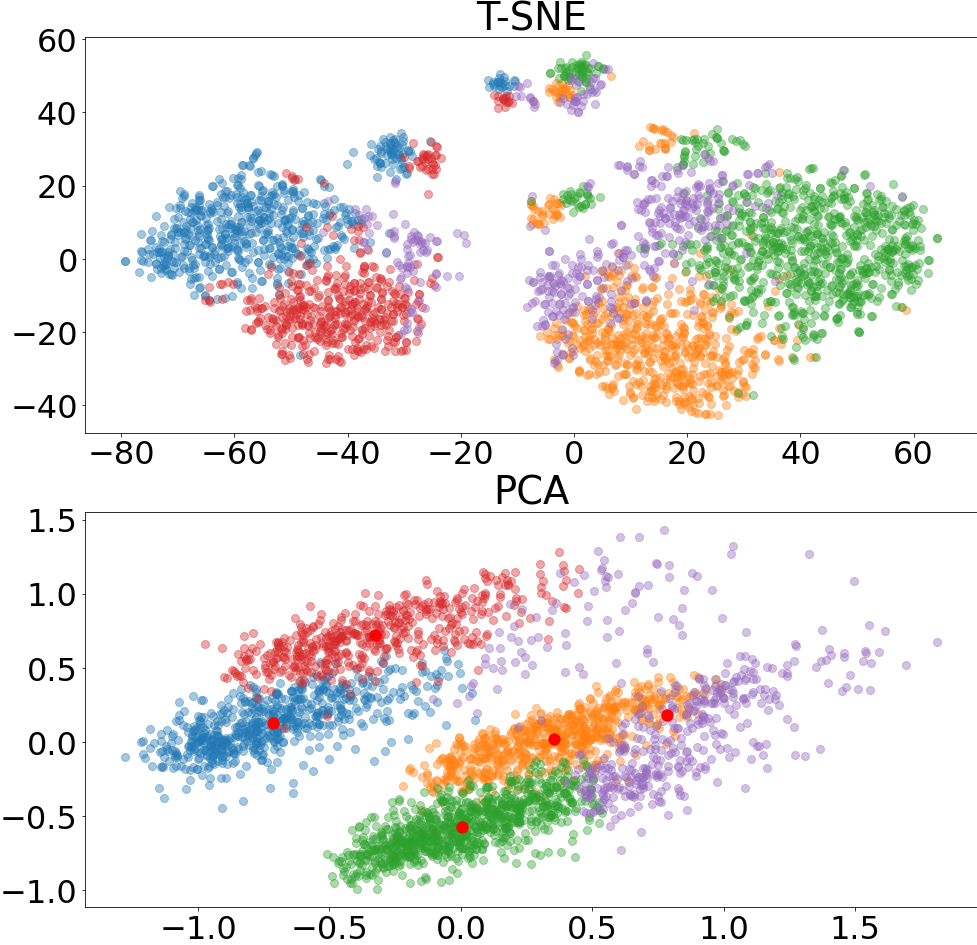
\includegraphics[width=\textwidth]{assests/5-means.png}
         \caption{5-Means}
         \label{fig:cluster:5means}
     \end{subfigure}
     \hfill
     \begin{subfigure}[b]{0.23\textwidth}
         \centering
         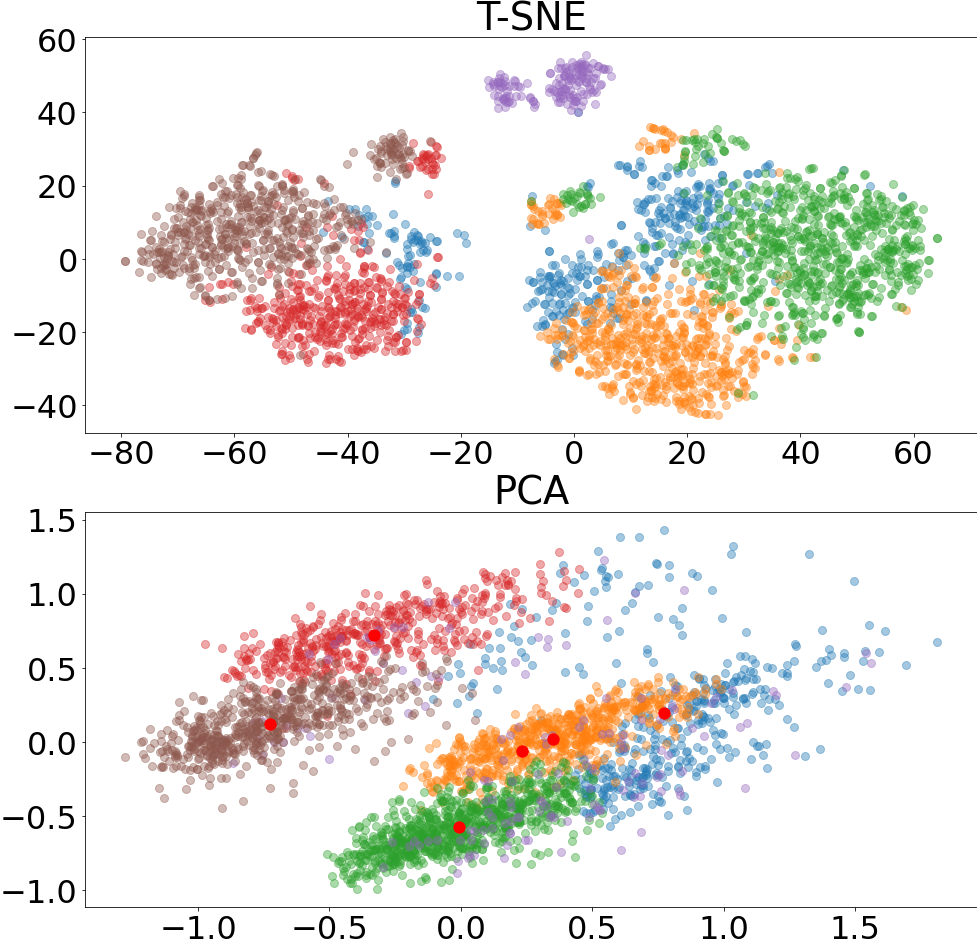
\includegraphics[width=\textwidth]{assests/6-means.png}
         \caption{6-Means}
         \label{fig:cluster:6means}
     \end{subfigure}
        \caption{Clustering results in the $2$-D space, using T-SEN (Top) and PCA (Bottom) for dimension reduction. The solid right point in PCA is the position of centroids.}
        \label{fig:cluster}
\end{figure*}

We adopt $K=6$ for the rest of this work as the overlapping on T-SEN graph is minimal.

The SSE (sum of squared error) of samples to their closest cluster center is $4698.20$, and $830.09, 850.01, 1127.67, 691.64, 325.35, 888.45$ for each cluster respectively with an average distance of $785.53$.

The cluster-SSE showed the statistical dispersion of each cluster.

There are generally two main cluster, labelled in (coffee and red), and (green and orange) respectively.
Each of them consists of two secondary cluster.
There are also two outliers marked in purple and blue.
The first one is hidden more in the linear space, but stick very closely in manifold.

\section{Findings}

In this work, we conduct extensive studies on a poll dataset of COVID-19 attitudes and behaviours in Australia~\cite{data}.

We used multiple algorithms to study different part of the dataset.

Limited by the population, the performance of modern deep learning algorithms is not ideal.
In specific, we construct a large transformer for satisfaction~\ref{satisfaction} with $220$ million parameters, while the dataset itself contains only $55$ features and $3061$ subjects.
The lack of time is also an important draw back.
We could have pretrained our transformer network, which would greatly improve the model performance.
And for opinionated~\ref{opinionated} and vote~\ref{vote}, we were unable to try different model and configure hyper-parameters, resulting an unsatisfactory result.

In the mean time, Decision Tree performs quite well in~\ref{opinionated}, achieving an AUROC socre of $1.0$.
This indicates that it could be useful for a preliminary result, especially for a small dataset like this.
Unfortunately, the Random Forest algorithm is never tested in this study, we anticipate it could achieve a better result.

The performance of SVM is not ideal in both opinionated~\ref{opinionated} and vote~\ref{vote}.
However, it takes no time to train and works well when data is properly processed,
making it an ideal choice in time-critical applications.

Although Logistic works in opinionated~\ref{opinionated} after data processing, we are unable to find it's advantages except for educational purpose.

%%%%%%%%% REFERENCES
{\small
\bibliographystyle{ieee_fullname}
\bibliography{bib}
}

\end{document}
